\section{ME21B079}
\subsection{Maxwell Equation}
\begin{center}
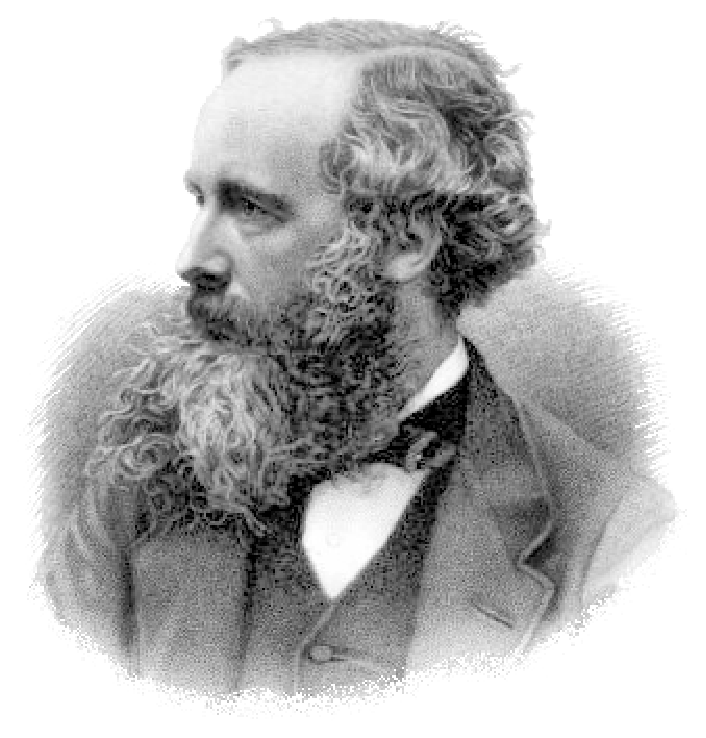
\includegraphics[width=0.5\textwidth]{./ME21B079/max.eps}
\end{center}
Faraday's law
$$ \frac{\partial\mathcal{D}}{\partial t} \quad  = \quad \nabla\times\mathcal{H}$$
Ampère's Law
$$ \frac{\partial\mathcal{B}}{\partial t} \quad  = \quad -\nabla\times\mathcal{E}$$
Gauss Law
$$ \nabla\cdot\mathcal{B}\quad  = \quad 0, \quad$$
Colomb's Law
$$ \nabla\cdot\mathcal{D}\quad  = \quad \rho_{v} $$
\subsection{Faraday's Law}
When the magnetic flux linking a circuit changes, an electromotive force is induced in the circuit proportional to the rate of change of the flux linkage.
\subsection{Ampère's Law}
The magnetic field created by an electric current is proportional to the size of that electric current with a constant of proportionality equal to the permeability of free space
\subsection{Gauss Law}
Gauss's law for magnetism states that the magnetic flux B across any closed surface is zero
\subsection{Colomb's Law}
The closed line integral of magnetic field vector is always equal to the total amount of scalar electric field enclosed within the path of any shape
\subsection{Expansion of variables}



\large\centering\begin{tabular}{ c c }  

  \textbf{'Symbol'} & \textbf{'Expansion'}  \\
    
  D & The volume of electric charge density \\   
  B & The magnetic field \\    
  E & The electric field \\    
  H & Magnetic field strength \\  
  
  $\rho$ & Free Charge Density\\
  

\large\centering\end{tabular}




